
% intro %

As its name suggests, high energy physics research is performed by studying subatomic particle collisions at very high energies.(fix me) 
%In high energy physics, we need two things: Accelerons to create particles and detectors to detect them.

The Large hadron collider (LHC) is one of the biggest accelerators we have today, and one of its general detectors is the Compact Muon Solenod (CMS) which is related to this thesis. This section provides details about the LHC, proton's journey toward the LHC. %and description of the CMS detector. 

%................................
\subsection{The large hadron collide}

LHC is the most powerful particle accelerator in the world. From its name “Large” refer to its big size which is about 27km in circumference and “Hadron" because it accelerates particles like protons or ions which are known as hadrons. Lastly, "Collider" because the particles traveling into two beams in opposite directions, are made to collide at four points around LHC ring.

The LHC is a part of the CERN accelerator complex and sits in a tunnel 100 meters underground at CERN, the European Organization for Nuclear Research, on the border of Switzerland and France near Geneva, Switzerland. Fig.~\ref{fig:LHC_location}

The CERN accelerator complex is a succession of machines where each machine accelerates a beam of particles to a given energy before injecting the beam into the next machine in the chain. LHC is the last element of this chain where it is designed to collide particles at COM energy up to 14 TeV. Fig.~\ref{fig:acceleration_complex}

The LHC is made of eight arcs and eight ‘insertions. The arcs contain the dipole ‘bending’ magnets. The layout of the straight section depends on the specific use of the insertion: physics (beam collisions within an experiment), injection, beam dumping or beam cleaning.

At the LHC we have 9 experiments: 
ALICE (study heavy ion collisions, QGP)  
ATLAS, CMS  (general purpose detectors)  
LHCb (study matter – antimatter asymmetry) 
 LHCf (shares intersection with ATLAS) 
TOTEM (shares intersection with CMS)  
MoEDAL-MAPP, (shares intersection with LHCb) 
FASER,SND@LHC.


\subsection{The journey of protons in the LHC}

It all starts from:  

- a compressed tank of hydrogen that is connected to source chamber of the linear accelerator. 
- The Linear accelerator 4 (Linac4) is designed to boost negative hydrogen ions (H with extra electron) to high energies (initial to 1/3 C)
- Then the particles are fed to the booster stage. (Proton Synchrotron Booster – PSB).at the PSB injection point a stripping foil will strip the electrons off the hydrogen anions creating protons that are accumulated as beam bunches in the four PSB rings. 
These proton bunches are then recombined at the exit of the PSB and further transferred down the CERN injector chain (accelerated to 91.6 of C).
- After that the beam is sent to Proton synchrotron (PS) where the increase of energy does not transfer to velocity. Instead, it will increase the relativistic mass (accelerated to 99.9 of C).
- Then the protons go to the super proton synchrotron. (SPS).
- Finally, at the LHC has two vacuum pipes where the protons will be going into different directions. 27 km ring of superconducting magnets (keep protons in the ring) that also has accelerating structures (radio frequency cavities) to boost the energy.  
- The LHC’s RF cavities bring the 450 GeV energy of the particles (1 GeV = 1 billion electron volts) to 6.5 TeV source. The maximum energy is reached in around 20 minutes with the bunches having passed through the RF cavities more than 10 million times. There are 4 points where the protons are collided. CMS is one of the them, where this thesis is focus on. 



 %------------ figures ------------%
\begin{figure}[t!]
\centering
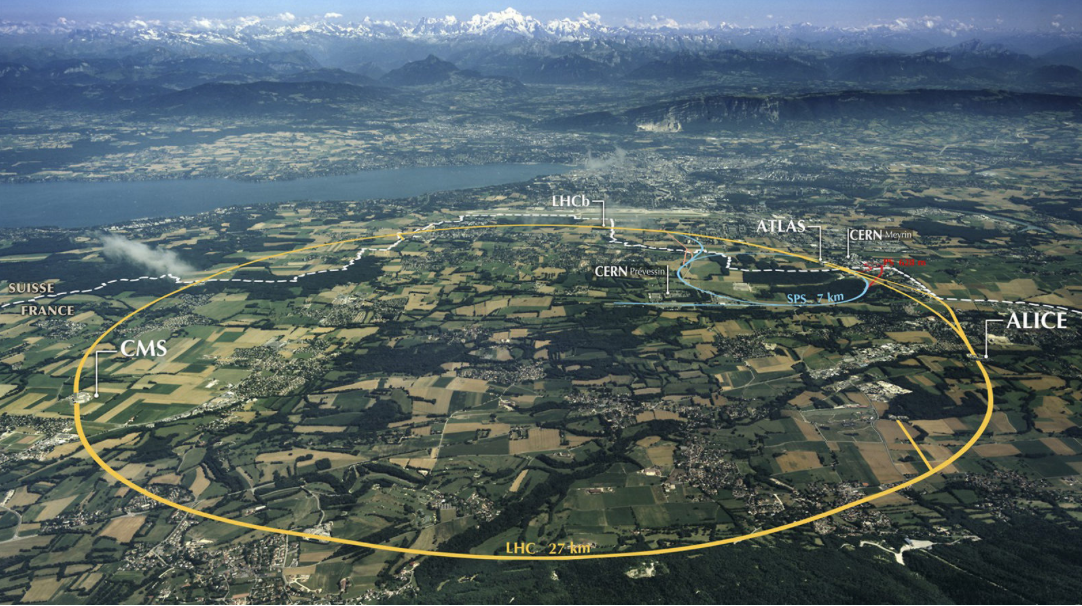
\includegraphics[width=0.99\textwidth]{figures/LHC_location.png}
\caption[location of the LHC]{location of the LHC}. Figure source~\cite{SMtable}.
\label{fig:LHC_location}
\end{figure}

\begin{figure}[t!]
\centering
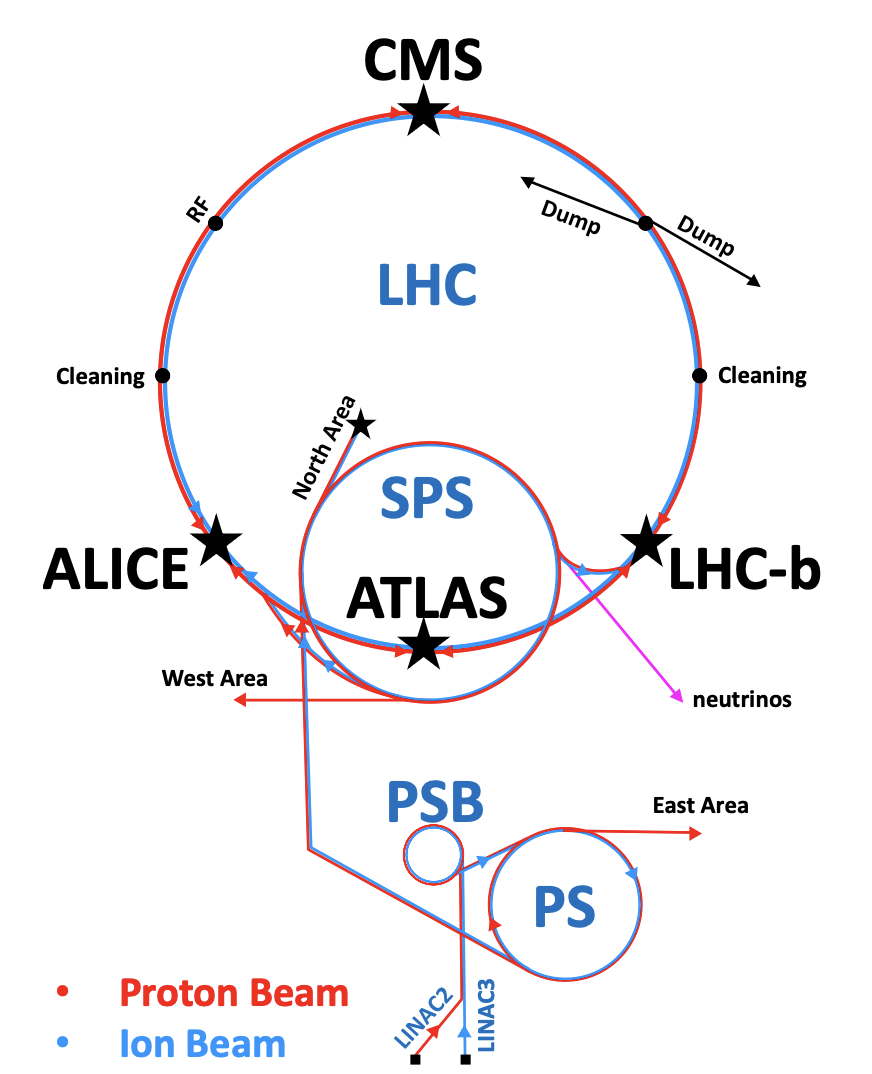
\includegraphics[width=0.99\textwidth]{figures/acceleration_chain.png}
\caption[acceleration complex]{acceleration complex}. Figure source~\cite{SMtable}.
\label{fig:acceleration_complex}
\end{figure} 
   

